% =============================================================================
% Master's thesis -- ENGLISH version
% Build:  tectonic main.tex     (or latexmk -pdf main.tex on Overleaf/TeXLive)
% =============================================================================
\documentclass[12pt, oneside]{report}

\usepackage[T1]{fontenc}
\usepackage[utf8]{inputenc}
\usepackage[english]{babel}

% =============================================================================
% Shared, language-neutral preamble.
% Each main.tex loads its documentclass + babel language FIRST, then \input's
% this file. Do NOT put \documentclass or babel here.
% =============================================================================

% --- Page geometry & spacing ---------------------------------------------------
\usepackage{geometry}
\geometry{a4paper, top=2.5cm, bottom=2.5cm, inner=3cm, outer=2.5cm}
\usepackage{setspace}
\onehalfspacing
\usepackage{microtype}

% --- Math ----------------------------------------------------------------------
\usepackage{amsmath, amssymb, mathtools}

% --- Graphics & figures --------------------------------------------------------
\usepackage{graphicx}
\graphicspath{{../common/figures/}{figures/}}
\usepackage{float}
\usepackage{caption}
\usepackage{subcaption}
\captionsetup{font=small, labelfont=bf}

% --- Tables --------------------------------------------------------------------
\usepackage{booktabs}
\usepackage{array}
\usepackage{tabularx}
\usepackage{longtable}
\usepackage{multirow}
\usepackage{siunitx}
\sisetup{group-separator={,}, group-minimum-digits=4, detect-weight=true, detect-family=true}

% --- Algorithms ----------------------------------------------------------------
\usepackage{algorithm}
\usepackage{algpseudocodex}

% --- Lists, color, misc --------------------------------------------------------
\usepackage{enumitem}
\usepackage{xcolor}
\definecolor{linknavy}{RGB}{20,60,110}

% --- Bibliography (biblatex + bibtex backend: compiles under tectonic; switch to
%     backend=biber on Overleaf for author-year/APA sorting if desired) ---------
\usepackage[backend=bibtex, style=ieee, sorting=nyt]{biblatex}
\addbibresource{../common/references.bib}

% --- Hyperlinks (load late) ----------------------------------------------------
\usepackage[hidelinks, breaklinks=true]{hyperref}
\hypersetup{colorlinks=true, linkcolor=linknavy, citecolor=linknavy, urlcolor=linknavy}
\usepackage[nameinlink]{cleveref}

% --- Project-specific shortcuts ------------------------------------------------
\newcommand{\ageb}{\textsc{ageb}\xspace}
\usepackage{xspace}
\renewcommand{\ageb}{\textsc{ageb}\xspace}
\newcommand{\nppv}{NPP--V\xspace}
\newcommand{\zmg}{ZMG\xspace}
\newcommand{\betadecay}{\ensuremath{\beta}}
\newcommand{\code}[1]{\texttt{#1}}

% Placeholder note for unfinished sections (visible but unobtrusive).
\newcommand{\todo}[1]{\medskip\noindent{\color{red!70!black}\small[\,TODO: #1\,]}\medskip}
\newcommand{\placeholder}{\todo{section to be written}}


% --- Thesis metadata (edit these) ---------------------------------------------
\newcommand{\thesistitle}{A Demand-Driven, Transferable Framework for Public
  Transit Corridor Prioritization and Generation}
\newcommand{\thesissubtitle}{A Node--Place--People Analysis of the Guadalajara
  Metropolitan Area}
\newcommand{\thesisauthor}{Alejandro Guevara}
\newcommand{\thesisadvisor}{Dr.~H\'ector G\'alvez}
\newcommand{\thesisprogram}{Master of Science in Data Science}
\newcommand{\thesisuniversity}{Universidad de Guadalajara}
\newcommand{\thesisfaculty}{Centro Universitario de Ciencias
  Econ\'omico Administrativas (CUCEA)}
\newcommand{\thesisyear}{2026}

\begin{document}

% ---- Front matter (roman page numbers) ----
\pagenumbering{roman}
\begin{titlepage}
\centering
\vspace*{1cm}

{\scshape\Large \thesisuniversity \par}
\vspace{0.5cm}
{\scshape \thesisprogram \par}
\vspace{2.5cm}

\rule{\linewidth}{0.4pt}\\[0.4cm]
{\huge\bfseries \thesistitle \par}
\vspace{0.4cm}
{\Large \thesissubtitle \par}
\rule{\linewidth}{0.4pt}\\[1.5cm]

{\Large\itshape \thesisauthor \par}
\vspace{2cm}

\begin{flushright}
\textit{Thesis advisor:}\\
\thesisadvisor
\end{flushright}

\vfill
{\large A thesis submitted in partial fulfillment of the requirements\\
for the degree of \thesisprogram \par}
\vspace{1cm}
{\large \thesisyear \par}

\end{titlepage}
\clearpage

\chapter*{Abstract}
\addcontentsline{toc}{chapter}{Abstract}

Conventional data-driven approaches to transit planning frequently predict where
transit \emph{already exists} rather than where it is \emph{needed}, producing
circular models that reward the status quo. This thesis develops a demand-driven,
transferable framework that instead diagnoses \emph{unmet} transit demand and
generates candidate corridors to address it, applied to the Guadalajara
Metropolitan Area (\zmg; \num{1881} census enumeration areas, \ageb, across ten
municipalities).

The framework proceeds in eight linked stages: (i)~a Tier-1 transit-demand surface
estimated from census, economic, and street-network data via a doubly-constrained
gravity model; (ii)~calibration of the distance-decay parameter against the 2022
Origin--Destination survey; (iii)~a supply layer measuring \textsc{gtfs}-based
accessibility and an independent \emph{coverage-gap} index that becomes the
supervised target, removing the circularity of ``has-a-stop'' labels; (iv)~a
Node--Place--People prioritization map with an explicit equity term; (v)~a formal
multi-objective evaluation function; (vi)~a corridor generator based on frontier
anchors, a minimum-spanning-tree diameter trunk, and an anchor-directness
feasibility gate; (vii)~an audit of the existing network; and (viii)~a validation
suite combining hold-out backtests, benchmarking, and before/after coverage
metrics.

The diagnostic layer is the strong contribution: the coverage-gap index is
corroborated out-of-sample by the 2025 opening of \zmg Line~4, whose corridor shows
\num{1.6} times the metropolitan high-gap rate. The generative layer produces at
least one substantive, feasible, merit-passing corridor while honestly
characterizing its limitations. Finally, the entire framework is transferred
end-to-end to two additional metropolitan areas of contrasting size---Toluca and
Aguascalientes---demonstrating that it is genuinely portable rather than bespoke to
\zmg.

\vspace{1em}
\noindent\textbf{Keywords:} public transit; travel demand; coverage gap; Node--Place
model; multi-objective optimization; equity; \textsc{gtfs}; transferability;
Guadalajara.

\clearpage

\chapter*{Acknowledgements}
\addcontentsline{toc}{chapter}{Acknowledgements}

\placeholder

\clearpage


\tableofcontents
\listoffigures
\listoftables
\clearpage

% ---- Body (arabic page numbers) ----
\pagenumbering{arabic}
\chapter{Introduction}
\label{ch:introduction}

\section{Motivation}
\label{sec:intro-motivation}

The Guadalajara Metropolitan Area (\zmg) faces the mobility predicament common to
large Latin American cities: a spatially-expanding, car-dependent periphery served by a
fragmented, largely concessioned bus system, onto which a small premium tier of bus
rapid transit and light rail has recently been grafted. In this setting the central
planning question is not how to describe the network that exists, but where new transit
would do the most good---which corridors carry latent, unmet demand that the current
supply fails to serve. Getting this question wrong is expensive: transit investment is
large, spatially fixed, and effectively irreversible once built.

\section{The circularity problem in data-driven transit planning}
\label{sec:intro-circularity}

A growing body of work applies machine learning to transit-network questions, typically
by training a model to predict where stations or stops ``should'' be. A recurring
methodological flaw undermines much of it: the dependent variable is derived, directly
or indirectly, from where transit \emph{already exists}. A model trained to predict a
``has-a-stop'' label, or a suitability class that is itself a function of current
supply, can only learn to reproduce the status quo. Such a model may report near-perfect
accuracy while being, by construction, incapable of identifying unmet need---it rewards
the network that already exists rather than diagnosing where it is absent. Breaking this
circularity is the methodological starting point of this thesis.

\section{Research questions}
\label{sec:intro-rqs}

The thesis is organized around four research questions:

\begin{description}
  \item[RQ1 -- Demand.] Can transit demand be estimated at \ageb resolution from
    Tier-1 (non-transit) data alone, so that demand is never a function of current
    supply?
  \item[RQ2 -- Diagnosis.] Does an independent coverage-gap index, built from demand
    against supply, identify genuinely under-served areas---and can it be validated
    out-of-sample?
  \item[RQ3 -- Generation.] Can candidate corridors be generated and evaluated on
    genuine need, non-redundancy, and demand efficiency, rather than on agreement with
    the existing network?
  \item[RQ4 -- Transferability.] Does the framework transfer to other metropolitan
    areas without bespoke re-engineering?
\end{description}

\section{Contributions}
\label{sec:intro-contributions}

The thesis makes four contributions, matched to the research questions. First, a
Tier-1 transit-demand surface (\cref{sec:w1}) that estimates latent demand without any
transit input, calibrated against a metropolitan travel survey. Second, and most
significantly, a \emph{coverage-gap diagnostic} (\cref{sec:w3,sec:w4}) that replaces the
circular ``has-a-stop'' target with an independent demand-versus-supply gap, and that is
corroborated out-of-sample by the subsequent opening of \zmg Line~4. Third, a corridor
generator and multi-objective evaluation (\cref{sec:w5,sec:w6}) that scores candidate
lines on need, non-redundancy, and demand efficiency, and that---once corridors are
shaped as real paths and judged by anchor-directness---produces at least one
substantive, feasible, merit-passing corridor. Fourth, a demonstration that the entire
framework \emph{transfers} end-to-end to two further metropolitan areas of contrasting
size (\cref{ch:transferability}). A cross-cutting contribution is methodological
honesty: the thesis distinguishes what it validates strongly (the diagnostic) from what
it validates only partially (the generator), and argues why the two carry different
evidential weight (\cref{ch:discussion}).

\section{Thesis structure}
\label{sec:intro-structure}

The remainder of the thesis follows the pipeline. \Cref{ch:literature} reviews the
Node--Place tradition, demand modeling, multi-criteria weighting, and machine-learning
siting, and locates the research gap. \Cref{ch:data} describes the study area, the
\ageb unit, and the data. \Cref{ch:methodology} presents the eight-workstream
framework in full. \Cref{ch:results} reports its outputs for \zmg, and
\cref{ch:transferability} repeats the analysis for Toluca and Aguascalientes.
\Cref{ch:discussion} interprets the results and their limits, and
\cref{ch:conclusions} answers the research questions and outlines future work.

\chapter{Theoretical Framework and Related Work}
\label{ch:literature}

\section{The Node--Place model and its extensions}
% Bertolini's Node-Place model; NP-RV / NPP-V extensions.
\placeholder

\section{Travel demand estimation}
% Four-step model; gravity / spatial-interaction models; doubly-constrained
% (Furness) balancing.
\placeholder

\section{Accessibility and coverage-gap analysis}
% Cumulative-opportunities accessibility; transit deserts / coverage gaps.
\placeholder

\section{Multi-criteria decision analysis and objective weighting}
% CRITIC and Entropy Weight Method; equity in transit prioritization.
\placeholder

\section{Machine learning for station and corridor siting}
% Random Forest / gradient boosting; SHAP interpretability; circular-target risk.
\placeholder

\section{Network design and corridor generation}
% Steiner-tree heuristics; minimum-spanning-tree approaches.
\placeholder

\section{Research gap}
\placeholder

\chapter{Study Area and Data}
\label{ch:data}

This chapter describes the study area, the spatial unit of analysis, and the data
that feed the pipeline. A recurring theme is data integrity: several of the results in
this thesis depend on corrections to the base geography and to specific indicators that
were discovered during a full reproducibility rebuild, and these are documented here so
that the numbers throughout are traceable.

\section{The Guadalajara Metropolitan Area}
\label{sec:area-zmg}

The primary study area is the Zona Metropolitana de Guadalajara (\zmg), Mexico's second
largest metropolitan area. Following the official delimitation, it comprises ten
municipalities of the state of Jalisco, spanning a dense central core (Guadalajara and
Zapopan) and a rapidly-urbanizing periphery (\cref{tab:munis}). Its mobility is marked
by high and rising car dependence, a large informally-operated concessioned bus system,
and, more recently, a small premium tier of bus rapid transit (Mi Macro) and light rail
(Mi Tren). This premium tier follows the wider Latin-American pattern in which bus rapid
transit has expanded rapidly as a cost-effective complement to rail
\parencite{hidalgo2013brt, cervero2013brt}; grafting it onto a largely concessioned base
network is precisely the setting that motivates a demand-driven rather than
supply-following approach to network planning.

\begin{table}[htbp]
\centering
\caption{The ten \zmg municipalities and their \ageb counts.}
\label{tab:munis}
\begin{tabular}{lS[table-format=3.0]}
\toprule
Municipality & {\ageb{}s} \\
\midrule
Zapopan                       & 481 \\
Guadalajara                   & 404 \\
Tlajomulco de Zúñiga          & 341 \\
San Pedro Tlaquepaque         & 213 \\
Tonalá                        & 207 \\
El Salto                      & 115 \\
Zapotlanejo                   & 41  \\
Ixtlahuacán de los Membrillos & 34  \\
Acatlán de Juárez             & 29  \\
Juanacatlán                   & 16  \\
\midrule
\textbf{Total}                & \textbf{1881} \\
\bottomrule
\end{tabular}
\end{table}

\section{The \ageb as unit of analysis}
\label{sec:area-ageb}

All indicators are aggregated to the \ageb (\emph{área geoestadística básica}), the
census enumeration area defined by INEGI. The \ageb is fine enough to resolve
intra-urban variation in demand and access, yet coarse enough that census attributes
are reported at its level. The analysis universe is restricted to urban \ageb{}s of the
ten \zmg municipalities: cells whose \code{CVE\_AGEB} carries an alphabetic suffix
(rural \ageb{}s) are excluded, as are all municipalities outside the metropolitan
delimitation. After this filter the universe is \num{1881} \ageb{}s
(\cref{tab:munis})---not the \num{2068} used in earlier drafts of this work, a
discrepancy explained in \cref{sec:area-integrity}.

\section{Data sources}
\label{sec:area-sources}

The pipeline deliberately separates \emph{Tier-1} data---census, economic, and
network variables available for any Mexican city---from the transit-supply data used
only to measure the coverage gap and to audit existing routes. \Cref{tab:data-sources}
lists the principal sources.

\begin{table}[htbp]
\centering
\caption{Principal data sources and their role in the pipeline.}
\label{tab:data-sources}
\begin{tabularx}{\linewidth}{llX}
\toprule
Source & Level & Role \\
\midrule
INEGI CPV2020    & \ageb / block & Population, youth share, vehicle ownership \\
DENUE            & establishment & Employment and POI attraction proxies \\
OpenStreetMap    & network       & Intersections, street density, drive graph \\
GTFS             & stop / route  & Existing accessibility and route audit \\
EOD 2022         & survey zone   & Gravity-model calibration \\
CONAPO / CONEVAL & \ageb         & Marginalization and social-lag (equity) \\
\bottomrule
\end{tabularx}
\end{table}

\begin{description}[leftmargin=1.4em, style=nextline]
  \item[Census and socio-demographics (INEGI CPV2020).] The 2020 population and
    housing census \parencite{inegi_cpv2020} supplies population, the youth share used to
    amplify trip generation, and household vehicle ownership (\code{VPH\_AUTOM} over
    \code{VIVPAR\_HAB}) used to derive transit propensity.
  \item[Economic activity (DENUE).] The national economic-unit directory
    \parencite{inegi_denue} provides establishment locations, aggregated to \ageb
    employment and point-of-interest and retail densities that drive trip attraction and
    accessibility opportunities.
  \item[Street network (OpenStreetMap).] The drive graph and derived Node indicators
    (intersection and street density) come from \textsc{osm} \parencite{openstreetmap},
    extracted for the ten municipalities with \textsc{osmnx} \parencite{boeing2017osmnx}.
  \item[Transit supply (GTFS).] The SITEUR \textsc{gtfs} feed defines the existing
    network used for the accessibility surface (\cref{sec:w3}) and the route audit
    (\cref{sec:w7}).
  \item[Origin--Destination survey (EOD 2022).] The 2022 metropolitan travel survey
    \parencite{imeplan_eod2022} provides observed zonal flows for calibrating the
    gravity model's distance decay (\cref{sec:w2}).
  \item[Equity indices (CONAPO, CONEVAL).] The marginalization index
    \parencite{conapo_marginacion2020} and the social-lag index
    \parencite{coneval_rezago2020} form the equity term (\cref{eq:equity}).
\end{description}

\section{Spatial conventions and data integrity}
\label{sec:area-integrity}

All computation uses the canonical projected reference system EPSG:6372 (Mexico
conic-equidistant); geographic coordinates (EPSG:4326) are used only for ingestion.
All geometry columns are spatially indexed.

A full from-scratch reproducibility rebuild surfaced three integrity defects that had
been silently present in earlier drafts, all now corrected. First, a municipality-code
typo in the base-geography filter had dropped an entire municipality on every rebuild;
fixing it, together with correctly excluding alphabetic-suffix \ageb{}s, gives the
\num{1881}-\ageb universe used throughout (earlier numbers computed against a
never-reproducible \num{2068}-row table should be read as superseded). Second, the
digital-elevation raster had been loaded under the wrong spatial reference, producing
geometrically meaningless slope values; the affected legacy model was retired rather
than re-run. Third, the marginalization index entered the equity term with an inverted
sign and an out-of-range zero-fill for unmatched \ageb{}s, which together had let the
equity bonus reward the \emph{least}-marginalized areas; correcting the direction and
using median imputation restores a monotonic, correctly-signed equity term. These
corrections materially affect several headline numbers and are the reason the results
in this thesis supersede any earlier figures for the same quantities.

\chapter{Methodology}
\label{ch:methodology}

This chapter presents the demand-driven framework in full. It is organized as
eight linked workstreams (\crefrange{sec:w1}{sec:w8}), summarized in
\cref{fig:pipeline}. The guiding design principle is a strict separation between a
\emph{diagnostic} layer (workstreams W1--W4), which estimates where transit is
needed independently of where it currently exists, and a \emph{generative and
validation} layer (W5--W8), which proposes and tests candidate corridors. All
spatial computation is performed in the canonical projected reference system
EPSG:6372, and all indicators are aggregated to the \ageb, the census enumeration
area used throughout as the unit of analysis.

\begin{figure}[htbp]
  \centering
  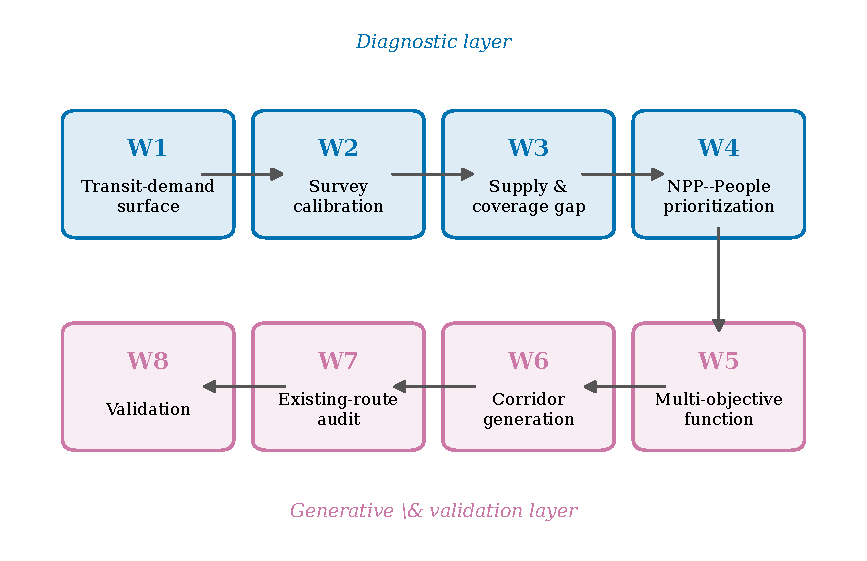
\includegraphics[width=\linewidth]{pipeline.pdf}
  \caption{The eight-workstream demand-driven framework. The diagnostic layer
    (W1--W4) is decoupled from existing supply; the generative and validation
    layer (W5--W8) proposes corridors and tests them.}
  \label{fig:pipeline}
\end{figure}

\section{Transit-demand estimation (W1)}
\label{sec:w1}

The framework begins by estimating a transit-demand surface from \emph{Tier-1}
data only---census, economic, and street-network variables---deliberately
excluding any existing-transit input so that demand is never a function of current
supply.

\subsection{Trip generation}
Daily trip productions $P_i$ for \ageb $i$ are estimated from population with a
youth-share amplification, reflecting the higher trip rates of younger cohorts:
\begin{equation}
  P_i = \tau \, \mathrm{pop}_i \,\bigl(1 + \gamma\, s^{\text{youth}}_i\bigr),
  \label{eq:productions}
\end{equation}
where $\tau = \num{2.5}$ trips per person per day and $\gamma = \num{0.10}$. Trip
attractions combine employment and activity proxies,
\begin{equation}
  A_i = w_e\, e_i + w_p\, \rho^{\text{poi}}_i a_i + w_r\, \rho^{\text{retail}}_i a_i,
  \label{eq:attractions}
\end{equation}
with $e_i$ the employment proxy, $\rho^{\text{poi}}_i$ and $\rho^{\text{retail}}_i$
point-of-interest and retail densities, and $a_i$ the \ageb area. The attraction
vector is then scaled so that $\sum_i A_i = \sum_i P_i$, a necessary condition for
the doubly-constrained model below.

\subsection{Doubly-constrained gravity model}
Origin--destination flows $T_{ij}$ are obtained from a doubly-constrained
spatial-interaction model \parencite{wilson1971gravity},
\begin{equation}
  T_{ij} = a_i\, b_j\, P_i\, A_j\, f(d_{ij}), \qquad
  f(d) = d^{-\beta},
  \label{eq:gravity}
\end{equation}
where $f$ is a power-law impedance on the Euclidean centroid distance $d_{ij}$ and
$\beta$ is the distance-decay parameter (calibrated in \cref{sec:w2}). The
balancing factors $a_i,b_j$ enforce the production and attraction constraints,
\begin{equation}
  a_i = \Bigl(\textstyle\sum_j b_j A_j f(d_{ij})\Bigr)^{-1}, \qquad
  b_j = \Bigl(\textstyle\sum_i a_i P_i f(d_{ij})\Bigr)^{-1},
  \label{eq:furness}
\end{equation}
solved by iterative proportional fitting (the Furness procedure), alternating the
two updates until the marginals converge (tolerance $10^{-5}$). Self-flows are
zeroed on the diagonal, and only pairs with $T_{ij}\ge\num{0.5}$ are retained in
the sparse output matrix.

\subsection{Transit-demand surface}
Total \ageb demand $D_i = \tfrac12\sum_j (T_{ij}+T_{ji})$ is finally weighted by a
transit-propensity term derived from household vehicle ownership. With
$v_i = \mathrm{VPH\_AUTOM}_i / \max(\mathrm{VIVPAR\_HAB}_i, 1)$ the vehicle rate,
\begin{equation}
  D^{\text{transit}}_i = D_i \,(1 - v_i),
  \label{eq:transit-demand}
\end{equation}
so that areas with high car ownership contribute proportionally less latent transit
demand. The resulting surface $D^{\text{transit}}$ is the dependent quantity that
drives the coverage-gap diagnosis in \cref{sec:w3}.

\section{Survey calibration (W2)}
\label{sec:w2}

The decay parameter $\beta$ is calibrated against the 2022 Origin--Destination
survey \parencite{imeplan_eod2022}. \ageb{}s are spatially joined to the survey's
traffic zones, modeled flows are aggregated to zone pairs, and $\beta$ is chosen to
minimize the sum of squared errors in log space between modeled and observed zonal
flows,
\begin{equation}
  \beta^\star = \arg\min_{\beta}\;
  \sum_{(z,z')} \Bigl(\log \hat{T}_{zz'}(\beta) - \log T^{\text{obs}}_{zz'}\Bigr)^2 .
  \label{eq:calibration}
\end{equation}
On the corrected \num{1881}-\ageb universe this yields $\beta^\star = \num{1.2005}$,
which outperforms the initial $\beta = \num{2.0}$ prior on both RMSE and $R^2$; the
calibrated value is adopted throughout.

\section{Supply and coverage-gap layer (W3)}
\label{sec:w3}

\subsection{Transit accessibility}
Existing supply is measured by a cumulative-opportunities accessibility surface
built from the \textsc{gtfs} feed. A directed transit graph is constructed from
consecutive stop pairs; from each \ageb, boarding stops within \SI{400}{\metre} are
identified, and a shortest-path search assigns to each reachable destination a
generalized travel time
\begin{equation}
  t = t_{\text{walk}} + t_{\text{wait}} + t_{\text{ivt}}
    = \frac{d_{\text{walk}}}{s_{\text{walk}}} + \frac{h}{2} + t_{\text{ivt}},
  \label{eq:traveltime}
\end{equation}
with walking speed $s_{\text{walk}} = \SI{80}{\metre\per\minute}$ and mean headway
$h$. Accessibility is the total employment reachable within a
\SI{45}{\minute} budget,
\begin{equation}
  \mathrm{Acc}_i = \sum_{j : t_{ij}\le 45} e_j .
  \label{eq:accessibility}
\end{equation}

\subsection{Coverage-gap index}
The core diagnostic combines demand and supply into a coverage-gap index,
\begin{equation}
  g_i = \frac{D^{\text{transit}}_i}{\mathrm{Acc}_i + \varepsilon},
  \qquad \varepsilon = 1,
  \label{eq:gap}
\end{equation}
normalized by a $\log(1+x)$ transform followed by min--max scaling to give
$g^{\,n}_i \in [0,1]$. \ageb{}s are then classified by joint quintiles: an \ageb is
\emph{High-gap} when it is in the top two demand quintiles and the bottom two
accessibility quintiles, \emph{Low-gap} in the mirror case, and \emph{Medium-gap}
otherwise. \Cref{fig:coverage-gap} maps the result for \zmg.

\begin{figure}[htbp]
  \centering
  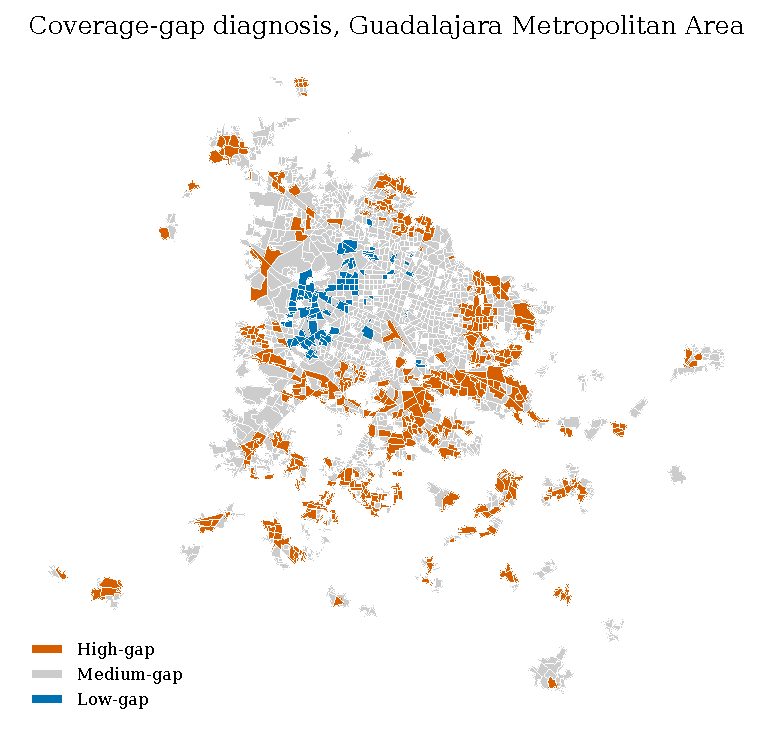
\includegraphics[width=0.82\linewidth]{zmg_coverage_gap.pdf}
  \caption{Coverage-gap diagnosis for the Guadalajara Metropolitan Area. The
    well-served core is Low-gap; High-gap \ageb{}s concentrate on the periphery.}
  \label{fig:coverage-gap}
\end{figure}

\subsection{Supervised model on the coverage-gap target}
To interpret the drivers of unmet demand, a binary target
$y_i = \mathbb{1}[g\text{-category}_i = \text{High-gap}]$ is regressed on the
\num{14} Node--Place--People indicators (all supply-side variables excluded to
prevent circularity) using Random Forest and gradient-boosted trees
\parencite{niu2023rf,ke2017lightgbm}. Model behaviour is interpreted with SHAP
values \parencite{lundberg2017shap}; population, social lag, and employment emerge
as the dominant drivers of High-gap status.

\section{Node--Place--People prioritization (W4)}
\label{sec:w4}

Independently of demand and supply, a place-based prioritization score is computed
from the \num{14} normalized indicators. Objective weights are derived without
expert input by combining the CRITIC method \parencite{diakoulaki1995critic} with
the Entropy Weight Method. The CRITIC weight of indicator $j$ rewards both
dispersion and independence,
\begin{equation}
  w^{\text{c}}_j \propto \sigma_j \sum_{k} \bigl(1 - r_{jk}\bigr),
  \label{eq:critic}
\end{equation}
with $\sigma_j$ the standard deviation of indicator $j$ and $r_{jk}$ its
correlation with indicator $k$; the two weightings are averaged into an ensemble
weight $w_j$ (\cref{fig:weights}). The place score, equity term, and final score
are
\begin{align}
  \mathrm{NPP}_i &= \textstyle\sum_j w_j\, x^{\,n}_{ij}, \label{eq:npp}\\
  \mathrm{Eq}_i  &= \tfrac12\bigl(x^{\,n,\text{marg}}_i + x^{\,n,\text{rezago}}_i\bigr),
    \label{eq:equity}\\
  F_i &= (1-\alpha)\,\mathrm{NPP}_i + \alpha\,\mathrm{Eq}_i, \qquad \alpha = 0.20.
  \label{eq:final}
\end{align}
The equity term is an explicit, separable additive bonus so that scores can be
reported with and without it; a sensitivity analysis over
$\alpha \in \{0.10, 0.20, 0.30\}$ confirms the ranking is robust
(Spearman $\ge 0.98$).

\begin{figure}[htbp]
  \centering
  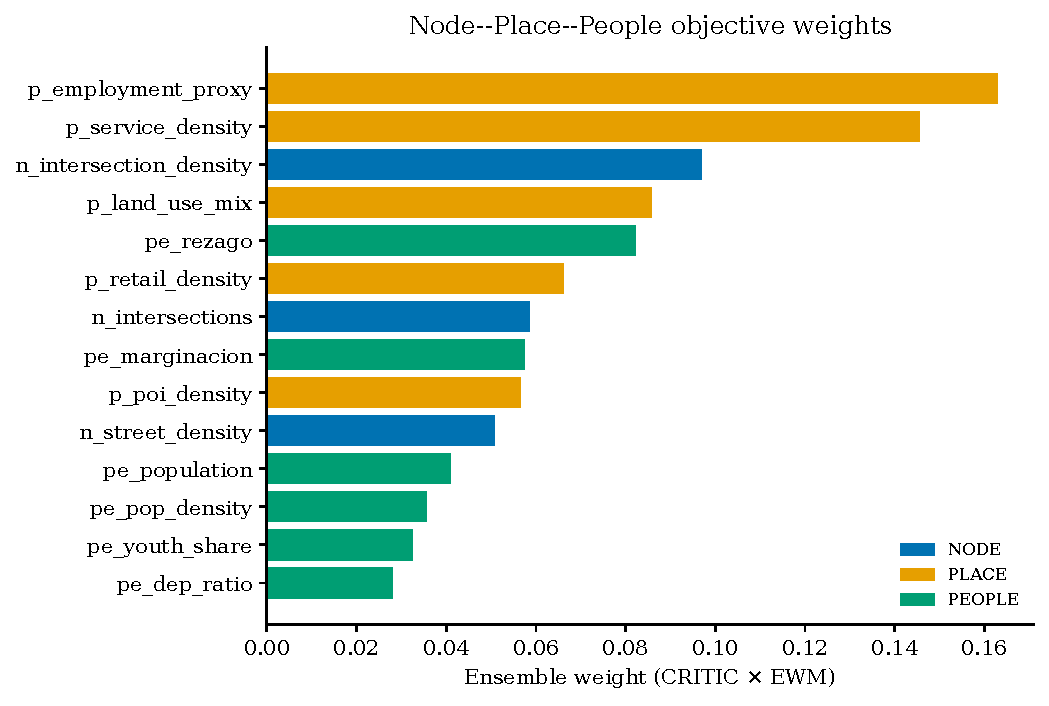
\includegraphics[width=0.85\linewidth]{w4_weights.pdf}
  \caption{Ensemble CRITIC$\,\times\,$EWM objective weights for the \num{14}
    Node--Place--People indicators, colored by dimension.}
  \label{fig:weights}
\end{figure}

\section{Multi-objective evaluation function (W5)}
\label{sec:w5}

Corridor candidates (from W6) and existing routes (in W7) are scored against three
competing objectives: demand-weighted gain $f_1$ (maximize), route length $f_2$
(minimize), and mean equity $f_3$ (maximize):
\begin{equation}
  f_1 = \frac{\sum_{i\in S} D_i\, \kappa\, u_i}{\sum_{i\in S} D_i}, \quad
  f_2 = \ell, \quad
  f_3 = \frac{1}{|S|}\sum_{i\in S}\mathrm{Eq}_i,
  \label{eq:objectives}
\end{equation}
where $S$ is the set of served \ageb{}s, $u_i = g^{\,n}_i$ the unserved fraction,
$\ell$ the route length, and $\kappa$ a gain factor ($\num{0.50}$ if the candidate
connects to the existing network, else $\num{0.20}$). A candidate is
\emph{feasible} only if it satisfies all constraints:
\begin{equation}
  \frac{\ell}{\ell_{\text{span}}} \le 1.8, \quad
  \frac{\ell\cdot 10^3}{n_{\text{stops}}-1} \in [300,1000]\,\si{\metre}, \quad
  \textstyle\sum_{i\in S} D_i \ge 500, \quad \ell \le \SI{30}{\kilo\metre},
  \label{eq:constraints}
\end{equation}
where $\ell_{\text{span}}$ is the straight-line span of the candidate's anchors (the
\emph{anchor-directness} denominator; see \cref{sec:w6}). Candidates are ranked by
non-dominated (Pareto) sorting minimizing $(-f_1, f_2, -f_3)$.

\section{Corridor generation (W6)}
\label{sec:w6}

New corridors are generated by \cref{alg:w6}. High-gap \ageb{}s are restricted to
the served/unserved \emph{frontier}---those within \SI{400}{\metre} of the existing
network---so that generated corridors intrinsically connect to it. Frontier anchors
are clustered spatially; within each cluster the corridor is the longest
leaf-to-leaf path (the \emph{diameter trunk}) of the anchors' minimum spanning tree,
stitched from real road segments of the drive graph. Feasibility uses the
anchor-directness ratio of \cref{eq:constraints} rather than an endpoint-detour
ratio, because the latter over-penalizes a demand-coverage corridor that
legitimately curves. Each feasible corridor is assigned a mode by demand threshold
(light rail $\ge \num{75000}$, bus rapid transit $\ge \num{15000}$, else local bus
trips per day). \Cref{fig:corridors} shows the four feasible \zmg corridors.

\begin{algorithm}[htbp]
\caption{Frontier-anchor corridor generation (W6)}
\label{alg:w6}
\begin{algorithmic}[1]
\Require coverage-gap surface $g^{\,n}$, demand $D$, drive graph $G$, network stops
\State $H \gets$ top Jenks class of $g^{\,n}$ with $D \ge 500$ \Comment{high-gap pool}
\State $H \gets \{i \in H : \operatorname{dist}(i,\text{network}) \le \SI{400}{\metre}\}$
  \Comment{frontier}
\State partition $H$ into $k$ spatial clusters by $k$-means
\ForAll{cluster $C$}
  \State $T \gets$ minimum spanning tree of $C$ on $G$
  \State $\pi \gets$ longest leaf-to-leaf path of $T$ \Comment{diameter trunk}
  \State build candidate from $\pi$; evaluate $f_1,f_2,f_3$ and constraints (W5)
\EndFor
\State \Return feasible candidates, Pareto-ranked
\end{algorithmic}
\end{algorithm}

\begin{figure}[htbp]
  \centering
  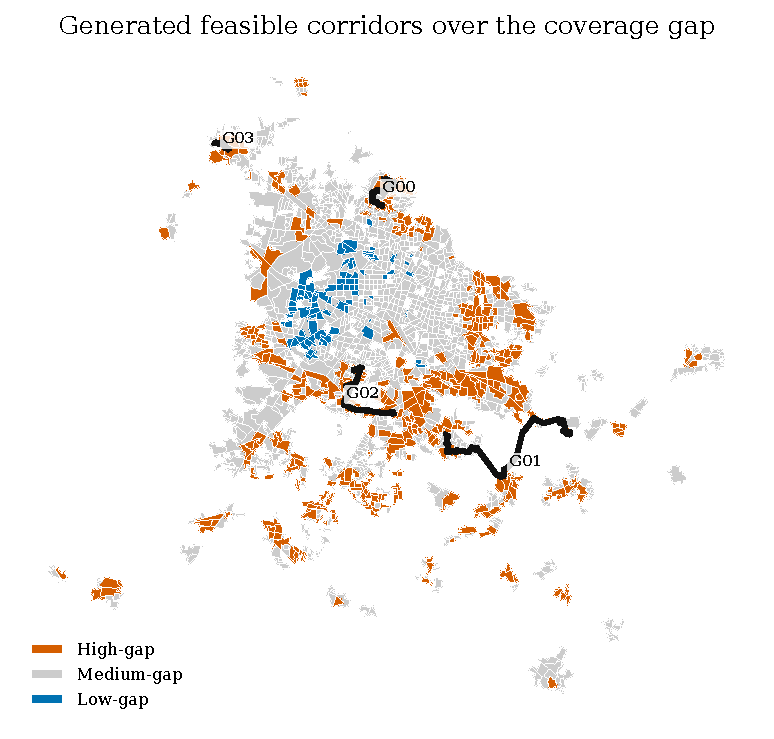
\includegraphics[width=0.82\linewidth]{zmg_corridors.pdf}
  \caption{The four feasible generated corridors (G00--G03) overlaid on the
    coverage-gap surface.}
  \label{fig:corridors}
\end{figure}

\section{Existing-route audit (W7)}
\label{sec:w7}

Every existing \textsc{gtfs} route is scored with the same W5 function and flagged
as \emph{Low demand} ($f_1<\num{0.2}$ and total score $<\num{0.3}$),
\emph{Indirect} (detour ratio $>\num{1.5}$), or \emph{Redundant} (served-\ageb
Jaccard overlap $\ge\num{0.60}$ with a higher-scoring route). Flagged routes receive
a modification proposal (shortcut, merge, or retire), making the audit directly
comparable to the generated corridors.

\section{Validation (W8)}
\label{sec:w8}

The framework is validated three ways. A \emph{hold-out backtest} masks the premium
transit tier from the \textsc{gtfs} feed, recomputes accessibility and the coverage
gap without it, re-runs the generator, and measures the shape overlap between
re-proposed corridors and the masked routes. A \emph{benchmark} compares the
generated corridors against existing premium routes. Finally, \emph{before/after
metrics}---coverage rate, the Gini coefficient of accessibility, and
population served per route-kilometre---quantify the marginal contribution of the
generated corridors. \Cref{ch:results} reports all three for \zmg and
\cref{ch:transferability} repeats them for the transfer cities.

\chapter{Results}
\label{ch:results}

This chapter reports the outputs of each workstream for the Guadalajara
Metropolitan Area (\zmg). Section order follows the pipeline: the estimated demand
surface (\cref{sec:res-w1}), its calibration (\cref{sec:res-w2}), the coverage-gap
diagnosis and its supervised interpretation (\cref{sec:res-w3}), the
Node--Place--People prioritization (\cref{sec:res-w4}), the generated corridors
(\cref{sec:res-w6}), the audit of the existing network (\cref{sec:res-w7}), and the
validation suite (\cref{sec:res-w8}).

\section{Estimated transit-demand surface (W1)}
\label{sec:res-w1}

The Tier-1 pipeline produces a transit-demand estimate for all \num{1881} \ageb{}s,
totalling \num{8471576} daily transit trip-ends. Household vehicle ownership varies
widely across the metropolis: the mean vehicle rate is \num{0.577}, giving a mean
transit propensity of \num{0.423}. Because demand is weighted by
$(1-v_i)$ (\cref{eq:transit-demand}), high-car-ownership \ageb{}s contribute
proportionally less latent transit demand even where raw trip generation is high.
\Cref{fig:demand} maps the resulting surface, which concentrates along the dense
central and eastern corridors of the metropolis.

\begin{figure}[htbp]
  \centering
  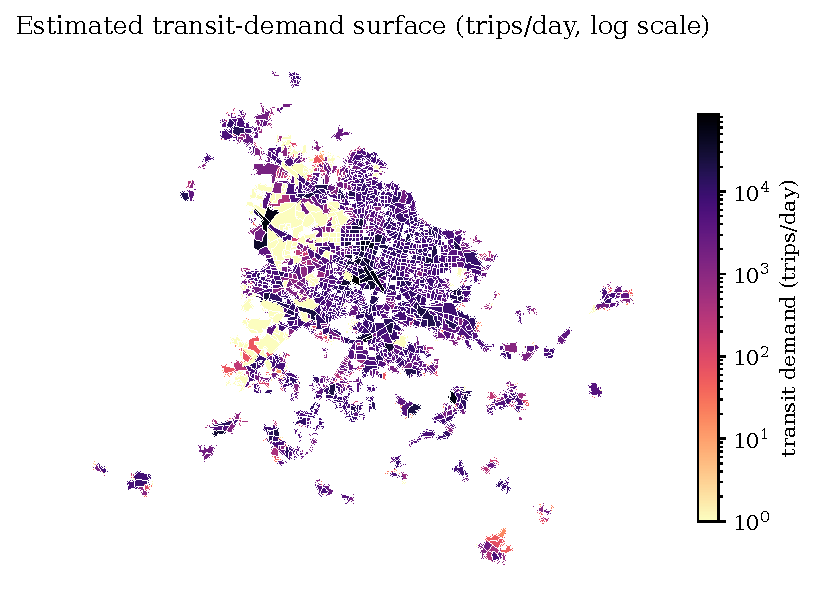
\includegraphics[width=0.82\linewidth]{zmg_demand.pdf}
  \caption{Estimated transit-demand surface (\ageb trips per day, log scale). Demand
    concentrates in the dense, lower-car-ownership central and eastern zones.}
  \label{fig:demand}
\end{figure}

\section{Gravity-model calibration (W2)}
\label{sec:res-w2}

Calibrating the distance-decay parameter against the 2022 Origin--Destination survey
(\cref{eq:calibration}) selects $\beta^\star = \num{1.2005}$, a markedly weaker decay
than the initial $\beta = \num{2.0}$ prior---\zmg commuters travel farther than the
prior assumed. Crucially, the calibrated value \emph{improves} fit on the corrected
\num{1881}-\ageb universe on every metric (\cref{tab:calibration}), reversing the
provisional conclusion drawn on the earlier, mis-filtered \ageb table. The calibrated
$\beta$ is adopted for the demand surface and all downstream workstreams.

\begin{table}[htbp]
\centering
\caption{Gravity-model calibration against the EOD 2022 survey.}
\label{tab:calibration}
\begin{tabular}{lS[table-format=4.1]S[table-format=1.4]}
\toprule
Model & {RMSE (trips)} & {$R^2$} \\
\midrule
Prior, $\beta = 2.0$        & 5088.2 & {--} \\
Calibrated, $\beta = 1.2005$ & 4524.9 & 0.2498 \\
\bottomrule
\end{tabular}
\end{table}

\section{Coverage-gap diagnosis (W3)}
\label{sec:res-w3}

Cumulative-opportunities accessibility (\cref{eq:accessibility}) combined with the
demand surface yields the coverage-gap index (\cref{eq:gap}). Classifying \ageb{}s by
joint demand/accessibility quintiles gives \num{390} High-gap (\SI{20.7}{\percent}),
\num{1413} Medium-gap, and \num{78} Low-gap areas (\cref{tab:gap}). As
\cref{fig:coverage-gap} showed, the High-gap areas form a periphery around a
well-served (Low-gap) core.

\begin{table}[htbp]
\centering
\caption{Coverage-gap classification of the \num{1881} \zmg \ageb{}s.}
\label{tab:gap}
\begin{tabular}{lS[table-format=4.0]S[table-format=2.1]}
\toprule
Category & {\ageb{}s} & {Share (\%)} \\
\midrule
High-gap   & 390  & 20.7 \\
Medium-gap & 1413 & 75.1 \\
Low-gap    & 78   & 4.1 \\
\bottomrule
\end{tabular}
\end{table}

Training a supervised model on the binary High-gap target (\cref{sec:w3}), with all
supply-side variables excluded, recovers the gap structure well and without leakage
(\cref{tab:retrain}). SHAP attribution ranks population, social lag
(\code{pe\_rezago}), and the employment proxy as the dominant drivers: High-gap areas
are dense, high-need, employment-rich zones that the current network under-serves.

\begin{table}[htbp]
\centering
\caption{Supervised retrain on the coverage-gap target (test fold).}
\label{tab:retrain}
\begin{tabular}{lS[table-format=1.3]S[table-format=1.3]}
\toprule
Model & {PR-AUC} & {ROC-AUC} \\
\midrule
Random Forest & 0.877 & 0.962 \\
LightGBM      & 0.883 & 0.962 \\
\bottomrule
\end{tabular}
\end{table}

\section{Node--Place--People prioritization (W4)}
\label{sec:res-w4}

The CRITIC$\,\times\,$EWM procedure (\cref{eq:critic}) assigns the largest objective
weights to the employment proxy (\num{0.163}), service density (\num{0.145}), and
four-way intersection density (\num{0.097}); the full weight vector appears in
\cref{fig:weights}. Averaged over all \ageb{}s, the place score is
$\overline{\mathrm{NPP}} = \num{0.4595}$, the equity term
$\overline{\mathrm{Eq}} = \num{0.2274}$, and the composite
$\overline{F} = \num{0.4131}$ at $\alpha = \num{0.20}$; the low equity mean is
expected, since \zmg is predominantly low-marginalization. A sensitivity analysis
over $\alpha \in \{0.10, 0.20, 0.30\}$ confirms the prioritization is robust: the
ranking correlates with the $\alpha = \num{0.20}$ baseline at Spearman
$\ge \num{0.98}$, so the equity weight shifts which specific \ageb{}s top the list
without disturbing the broad structure.

\section{Generated corridors (W6)}
\label{sec:res-w6}

The generator produces five candidate corridors, of which four are feasible
(\cref{tab:corridors}); the fifth (\code{W6\_G05}) is rejected on the
anchor-directness constraint (\num{1.93} > \num{1.8}). \Cref{fig:corridors} maps the
four feasible corridors over the coverage-gap surface, and \cref{fig:pareto} places
all candidates in objective space.

\begin{table}[htbp]
\centering
\caption{Generated corridor candidates. \code{W6\_G05} fails the anchor-directness
  constraint.}
\label{tab:corridors}
\begin{tabular}{l S[table-format=2.1] S[table-format=2.0] S[table-format=6.0] l c}
\toprule
Corridor & {km} & {\ageb{}s} & {Demand/day} & Mode & Feasible \\
\midrule
W6\_G00 & 7.3  & 18 & 66041  & BRT             & Yes \\
W6\_G01 & 23.0 & 27 & 96839  & Light rail      & Yes \\
W6\_G02 & 12.1 & 25 & 192357 & Light rail      & Yes \\
W6\_G03 & 2.4  & 5  & 35784  & BRT             & Yes \\
W6\_G05 & 5.4  & 14 & 80234  & Light rail      & {--} \\
\bottomrule
\end{tabular}
\end{table}

\begin{figure}[htbp]
  \centering
  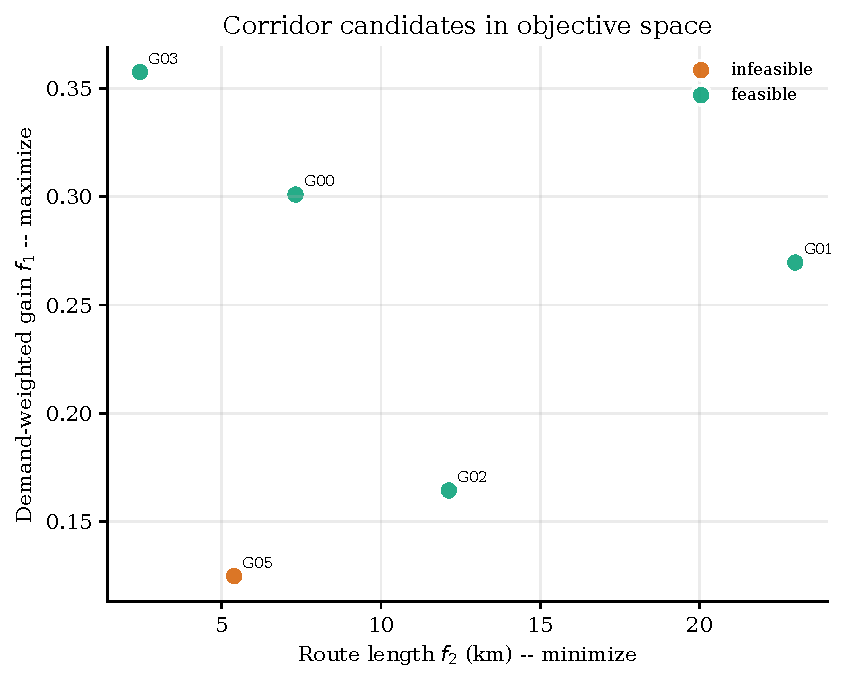
\includegraphics[width=0.78\linewidth]{w6_pareto.pdf}
  \caption{Corridor candidates in $(f_2, f_1)$ objective space, colored by
    feasibility. Feasible corridors span a range of length/gain trade-offs.}
  \label{fig:pareto}
\end{figure}

The stand-out result is \code{W6\_G02}: a substantive \SI{12.1}{\kilo\metre},
\num{25}-\ageb corridor carrying an estimated \num{192357} trips/day. On the merit
tests introduced for validation (\cref{sec:res-w8}) it is the only feasible corridor
that passes all three: \SI{56}{\percent} of its served \ageb{}s are High-gap (versus
the \SI{20.7}{\percent} metropolitan baseline), it is non-redundant with existing
routes (best Jaccard \num{0.18}), and its demand per kilometre sits at the
\num{73}rd percentile of the existing network. \code{W6\_G03} also passes but is a
short \SI{2.4}{\kilo\metre} stub, while \code{W6\_G00} and \code{W6\_G01} serve real
need yet are lower-efficiency connectors---a mixed but honestly characterized
outcome discussed in \cref{ch:discussion}.

\section{Existing-route audit (W7)}
\label{sec:res-w7}

Scoring all \num{247} existing SITEUR routes with the same multi-objective function
flags \num{229} of them (\cref{tab:audit}): \num{109} as Indirect, \num{80} as Low
demand, and \num{40} as Redundant, leaving only \num{18} unflagged.
\Cref{fig:w7audit} plots every route in objective space by flag. Each flagged route
carries a modification proposal (shortcut, merge, or retire), making the audit
directly comparable to the generated corridors.

\begin{table}[htbp]
\centering
\caption{Audit flags across the \num{247} existing SITEUR routes.}
\label{tab:audit}
\begin{tabular}{lS[table-format=3.0]}
\toprule
Flag & {Routes} \\
\midrule
Indirect   & 109 \\
Low demand & 80 \\
Redundant  & 40 \\
Unflagged  & 18 \\
\bottomrule
\end{tabular}
\end{table}

\begin{figure}[htbp]
  \centering
  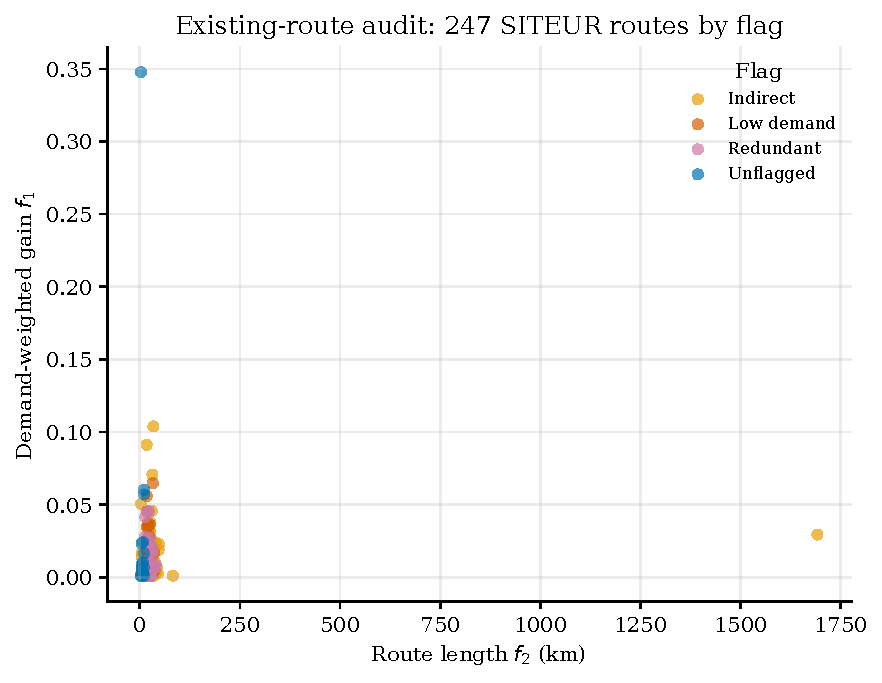
\includegraphics[width=0.82\linewidth]{w7_audit.pdf}
  \caption{Existing-route audit: the \num{247} SITEUR routes in $(f_2, f_1)$ space,
    colored by audit flag.}
  \label{fig:w7audit}
\end{figure}

\section{Validation (W8)}
\label{sec:res-w8}

\paragraph{Hold-out backtest and benchmark.} Masking the premium tier (Mi Macro and
Mi Tren) and re-running the generator reproduces the masked routes with a mean
shape overlap of only \SI{15.0}{\percent}; masking individual rail lines yields
\SI{0}{\percent}. The benchmark against \num{33} existing premium routes gives a
mean overlap of \SI{10.5}{\percent} for \SI{44.9}{\kilo\metre} of generated
corridor. Low overlap is the expected and desired outcome: the generator identifies
genuinely under-served areas rather than replicating existing lines. Reconstruction
is, in any case, a weak proxy for corridor merit (\cref{ch:discussion}).

\paragraph{Before/after metrics.} Adding the feasible corridors to the existing
network improves every coverage metric (\cref{tab:beforeafter}): the \ageb coverage
rate rises by \num{1.1} percentage points, the accessibility Gini falls by
\num{0.0187}, and \num{47} previously-unserved \ageb{}s---home to \num{120648}
people---gain service.

\begin{table}[htbp]
\centering
\caption{Before/after coverage metrics for the feasible W6 corridors.}
\label{tab:beforeafter}
\begin{tabular}{lS[table-format=2.1]S[table-format=2.1]S[table-format=+1.4]}
\toprule
Metric & {Before} & {After} & {$\Delta$} \\
\midrule
Coverage rate (\%)  & 69.9   & 71.0   & +1.1 \\
Accessibility Gini  & 0.6333 & 0.6146 & -0.0187 \\
\bottomrule
\end{tabular}
\end{table}

\paragraph{Out-of-sample corroboration.} The strongest validation is external: the
2024 \textsc{gtfs} snapshot predates the December~2025 opening of SITEUR Line~4, so
the diagnostic treats the Line~4 corridor as unserved. Its \ageb{}s show
\num{1.6} times the metropolitan High-gap rate, confirming out-of-sample that the
coverage-gap index flags corridors that planners independently chose to build. This
corroborates the \emph{diagnostic} layer; it does not prove the generator would have
produced Line~4, a distinction developed in \cref{ch:discussion}.

\chapter{Transferability}
\label{ch:transferability}

A framework that works only for the city it was built on is of limited scientific
value. This chapter tests research question RQ4 by transferring the entire pipeline
to two further metropolitan areas through a single parameterized code path, and
asks whether the diagnostic, generative, and validation layers all survive the move.

\section{Study design}
\label{sec:transf-design}

Two transfer cities were chosen to bracket \zmg in size and structure:
\textbf{Toluca} (Zona Metropolitana del Valle de Toluca, \num{16} municipalities,
$\sim$\num{2.3} million inhabitants, \num{538} urban \ageb{}s) as a large metro
comparable to \zmg, and \textbf{Aguascalientes} (\num{3} municipalities, \num{356}
urban \ageb{}s) as a compact one. Monterrey was the original target but its
\textsc{gtfs} feed proved unobtainable, which blocks the supply layer; it is retained
only as a Tier-1 (demand-only) reference. Both transfer cities have verified,
downloadable \textsc{gtfs}.

Every stage runs through the same code as \zmg, invoked as
\code{w9\_run\_*.py -{}-city \{tol,ags\}}, reusing the pure \zmg functions over
per-city configuration. Tier-1 inputs (census, \textsc{denue}, street network) are
national and therefore available everywhere; equity indices come from the same
CONAPO and CONEVAL products. No local Origin--Destination survey exists for either
city, so the calibrated $\beta = \num{1.2005}$ is transferred from \zmg; because the
size-comparison metrics below are ratios, they are insensitive to this choice.

\section{Demand and coverage-gap transfer}
\label{sec:transf-diagnosis}

The demand surface transfers cleanly and, more importantly, \emph{differentiates} the
three cities in interpretable ways (\cref{tab:transfer-diag}, \cref{fig:transfer}).
Mean household vehicle ownership follows a clear gradient---Toluca \num{0.529} $<$
\zmg \num{0.577} $<$ Monterrey \num{0.635} (Tier-1 reference) $<$ Aguascalientes
\num{0.667}---so the least car-dependent metro is the large, lower-income Toluca and
the most car-dependent is compact, higher-income Aguascalientes.

\begin{table}[htbp]
\centering
\caption{Diagnostic transfer across the three \textsc{gtfs} cities.}
\label{tab:transfer-diag}
\begin{tabular}{l S[table-format=4.0] S[table-format=1.3] S[table-format=2.1] S[table-format=2.1]}
\toprule
City & {Urban \ageb{}s} & {Vehicle rate} & {Unserved (\%)} & {High-gap (\%)} \\
\midrule
Guadalajara    & 1881 & 0.577 & 32.7 & 20.7 \\
Toluca         & 538  & 0.529 & 19.1 & 14.9 \\
Aguascalientes & 356  & 0.667 & 19.7 & 9.6 \\
\bottomrule
\end{tabular}
\end{table}

The coverage-gap diagnosis likewise transfers and orders the cities sensibly: the
High-gap share is highest in \zmg (\SI{20.7}{\percent}), lower in Toluca
(\SI{14.9}{\percent}), and lowest in the compact, well-covered Aguascalientes
(\SI{9.6}{\percent}). The diagnostic is thus not a \zmg artifact---it produces a
plausible, differentiated reading of unmet demand in every metro.

\begin{figure}[htbp]
  \centering
  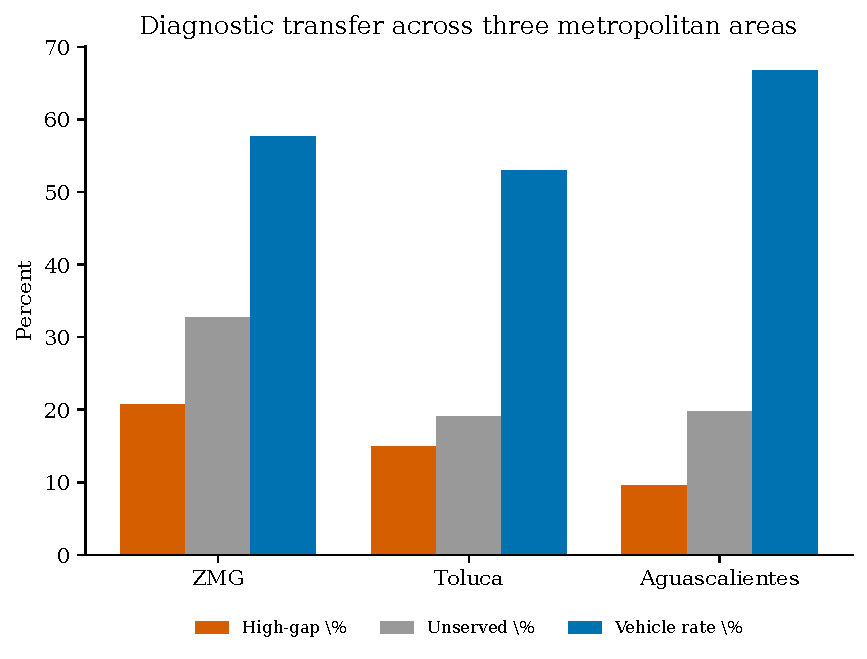
\includegraphics[width=0.85\linewidth]{transfer_highgap.pdf}
  \caption{Diagnostic transfer: High-gap share, unserved share, and mean vehicle
    rate across the three metropolitan areas.}
  \label{fig:transfer}
\end{figure}

\section{Prioritization and corridor generation transfer}
\label{sec:transf-generation}

The Node--Place--People weighting re-derives its own weights per city rather than
importing \zmg's. Notably, \emph{social lag} (\code{pe\_rezago}) becomes the single
largest objective weight in both transfer cities (Toluca \num{0.182}, Aguascalientes
\num{0.247}), whereas in \zmg the employment and population terms led. Because the
weights are data-driven (CRITIC$\,\times\,$EWM), this shift is a feature: the method
adapts its emphasis to each city's own indicator structure.

Corridor generation produces substantive, feasible corridors in both cities
(\cref{tab:transfer-corridors}). Toluca's best feasible corridor, \code{W6\_G01}
(\SI{12.6}{\kilo\metre}, \num{23} \ageb{}s, \num{133728} trips/day, light rail), is
the direct transfer analogue of \zmg's merit-passing \code{W6\_G02}. Aguascalientes
yields \code{W6\_G05} (\SI{5.9}{\kilo\metre}, \num{12} \ageb{}s, \num{107633}
trips/day). The same feasibility-versus-directness signature seen in \zmg reappears:
in Aguascalientes a genuinely high-demand corridor (\code{W6\_G03}, \num{22}
\ageb{}s, \num{115162} trips/day) is rejected for exceeding the directness cap
(\num{2.03} > \num{1.8})---the identical behaviour documented for \zmg, now observed
in a different city.

\begin{table}[htbp]
\centering
\caption{Best feasible corridor per transfer city, with the notable infeasible case.}
\label{tab:transfer-corridors}
\begin{tabular}{ll S[table-format=2.1] S[table-format=2.0] S[table-format=6.0] c}
\toprule
City & Corridor & {km} & {\ageb{}s} & {Demand/day} & Feasible \\
\midrule
Toluca         & W6\_G01 & 12.6 & 23 & 133728 & Yes \\
Aguascalientes & W6\_G05 & 5.9  & 12 & 107633 & Yes \\
Aguascalientes & W6\_G03 & 13.9 & 22 & 115162 & {--} \\
\bottomrule
\end{tabular}
\end{table}

\section{Validation transfer}
\label{sec:transf-validation}

The audit and validation layers transfer as well, with one honest exception. The W7
audit runs on both networks (\cref{tab:transfer-audit}). Toluca's \num{622}
concessioned routes are flagged almost universally---\num{612} of \num{622}, of which
\num{431} are Redundant---quantifying the parallelism of a system with roughly thirty
operators. (Its zero feasible count is a source-\textsc{gtfs} artifact: median stop
spacing is \SI{43}{\metre}, far below the \SI{300}{\metre} constraint, so the
audit's flags rather than its feasibility gate carry the signal.) Aguascalientes,
with \num{48} routes at \SI{239}{\metre} spacing, has \num{6} feasible routes and
\num{47} flagged.

\begin{table}[htbp]
\centering
\caption{Existing-route audit (W7) for the transfer cities.}
\label{tab:transfer-audit}
\begin{tabular}{l S[table-format=3.0] S[table-format=3.0] S[table-format=3.0] S[table-format=2.0] S[table-format=2.0]}
\toprule
City & {Routes} & {Flagged} & {Redundant} & {Indirect} & {Low dem.} \\
\midrule
Toluca         & 622 & 612 & 431 & 88 & 93 \\
Aguascalientes & 48  & 47  & 4   & 33 & 10 \\
\bottomrule
\end{tabular}
\end{table}

The W8 benchmark reveals a genuine transferability insight. In both transfer cities
the generated corridors overlap the existing network \emph{heavily}---Toluca
\SI{75.0}{\percent}, Aguascalientes \SI{54.3}{\percent}---the opposite of \zmg's low
overlap. In these already well-served networks ($\sim$\SI{80}{\percent} baseline
coverage) the highest-demand corridors are already served, so the generator
\emph{re-identifies} them (revealed-preference corroboration) rather than opening new
coverage; correspondingly, the before/after gains are modest (Toluca coverage
$+\num{0.4}$~pp, Gini $-\num{0.0031}$; Aguascalientes $+\num{0.3}$~pp,
$-\num{0.0027}$).

The mask-and-reconstruct backtest, however, does \emph{not} transfer to a bus-only
network. Neither city has a premium tier to hold out. A demand-trunk proxy applied to
Toluca (masking the \num{23} busiest routes) collapses: frontier anchors fall from
\num{14} to \num{6} and no multi-anchor corridor can form, so nothing is re-proposed.
The mechanism is intrinsic---\zmg's premium rail is a separable overlay redundant with
parallel buses, so masking it leaves the served/unserved seam intact, whereas a bus
trunk \emph{is} the local service and masking it erases the seam the generator depends
on. This is a documented precondition of the backtest, not a defect of the framework;
the benchmark and before/after metrics remain the operative validation for cities
without a premium tier.

\section{Transfer error and limitations}
\label{sec:transf-limits}

Four caveats bound the transfer claim. First, \textbf{no local calibration}: $\beta$
is transferred from \zmg, so absolute demand magnitudes carry the prior's error,
though the ratio-based diagnostics do not. Second, \textbf{a coarser equity input}:
CONEVAL publishes only a categorical social-lag \emph{grade} at \ageb level for 2020,
so \code{pe\_rezago} is an ordinal approximation of \zmg's continuous index
(direction preserved, granularity coarser). Third, \textbf{unit-scale incomparability}:
the \ageb is much coarser relative to population in semi-rural Toluca, so cross-city
\ageb counts are not directly comparable and only per-\ageb and per-capita metrics
are. Fourth, as shown above, \textbf{the hold-out backtest requires a premium tier}
that bus-only networks lack. None of these undermines the central result: the
complete framework transfers end-to-end to two metros of very different size through
one code path, on cities Monterrey's missing feed had made impossible.

\chapter{Discussion}
\label{ch:discussion}

The results support a deliberately bounded claim. This chapter separates what the
framework demonstrates strongly from what it demonstrates only partially, and argues
that the distinction turns on two different questions that prior work often conflates.
The central thesis is this: the framework contributes a \emph{validated demand-gap
diagnostic} and a \emph{characterized, partially-successful corridor generator}, and
these two contributions carry different evidential weight.

\section{Two questions, two layers}
\label{sec:disc-twoquestions}

It is useful to distinguish two questions that a data-driven planning framework might
be asked to answer. Question~A: does the generator \emph{reproduce corridors that were
actually built}? Question~B: does the generator \emph{produce good corridors}---lines
that serve real, unmet demand efficiently and without redundancy? Much of the
literature on machine-learning station siting implicitly answers a version of
Question~A, treating agreement with the existing network as validation. But A is a
weak and asymmetric proxy for B, because built lines are not guaranteed to be optimal:
they are chosen under political, financial, and land-availability constraints that the
framework does not model. Agreement therefore corroborates; disagreement is faint
evidence of error. The two pipeline layers map onto these questions---the diagnostic
layer (W1--W4) is validated against B-type evidence, while the generator (W5--W6) is
tested against both---and they succeed to different degrees.

\section{The diagnostic layer is the strong contribution}
\label{sec:disc-diagnostic}

The coverage-gap diagnosis (\cref{ch:methodology}, \cref{sec:w3}) is the framework's
firmest result. Its methodological contribution is to break the circularity that
undermines ``has-a-stop'' targets: by defining the dependent variable as the ratio of
independently-estimated demand to \textsc{gtfs}-measured supply
(\cref{eq:gap}), the model learns where transit is \emph{needed} rather than where it
\emph{exists}. The supervised retrain confirms this target is learnable from
place characteristics alone, with no supply-side leakage (\cref{tab:retrain}).

Three lines of evidence support the diagnostic. First, and most importantly, it is
corroborated \emph{out of sample}: the 2024 \textsc{gtfs} snapshot predates SITEUR
Line~4, so the corridor is treated as unserved, yet its \ageb{}s show \num{1.6} times
the metropolitan High-gap rate (\cref{sec:res-w8}). A corridor that professional
planners independently chose to build was flagged as high-priority by the model that
never saw it. Second, the diagnostic \emph{transfers}: it produces a plausible,
differentiated reading of unmet demand in two further cities (\cref{ch:transferability}),
ordering them sensibly by High-gap share. Third, it is \emph{interpretable}: SHAP
attribution identifies dense, high-need, employment-rich but under-served zones,
matching the geographic pattern in \cref{fig:coverage-gap}. This layer is the
defensible, citable core of the thesis.

\section{The generative layer is a characterized, partial success}
\label{sec:disc-generative}

The corridor generator is a weaker but genuine contribution, and its history is
instructive. In its first form the generator was essentially negative: of its feasible
corridors, only a degenerate short stub passed the merit tests, and feasibility was
confounded with anchor-cluster sparsity---the feasibility filter selected for
\emph{few, near-collinear anchors} rather than for good corridors. This was traced to
two coupled defects: a shaper that flattened a minimum spanning tree into a line with
phantom jumps, and a detour metric measured against the endpoint distance, which
over-penalizes a demand-coverage corridor that legitimately curves.

Re-architecting the generator around frontier anchors, a minimum-spanning-tree
\emph{diameter} trunk stitched from real roads, and an \emph{anchor-directness}
feasibility gate (\cref{sec:w6}) changed the verdict. On its own terms the generator
now produces at least one substantive, feasible, merit-passing corridor:
\code{W6\_G02} serves \SI{12.1}{\kilo\metre} and \num{25} \ageb{}s, of which
\SI{56}{\percent} are High-gap (versus the \SI{20.7}{\percent} baseline), is
non-redundant with the existing network (best Jaccard \num{0.18}), and sits at the
\num{73}rd percentile of demand per kilometre. This is a real line, not a stub.

The success is partial, however, and the thesis does not overstate it. Alongside
\code{W6\_G02}, the generator also surfaces lower-efficiency connectors
(\code{W6\_G00} and \code{W6\_G01}) that serve real need but rank poorly on demand per
kilometre. The residual limitation is architectural---the fixed anchor count, spatial
clustering, and spanning-tree trunk cannot target every high-gap pocket---and it is
now measured rather than merely asserted.

\section{Reconstruction is a weak proxy for corridor merit}
\label{sec:disc-reconstruction}

The clearest illustration of the Question-A/Question-B distinction is the generator's
failure to reconstruct built rail. Across masked backtests it does not re-discover the
premium lines: masking the whole premium tier yields \SI{15}{\percent} mean shape
overlap, and masking individual rail lines yields essentially zero
(\cref{sec:res-w8}); the Line~4 corridor is matched at only \num{0.05} recall. Taken
naively, this looks like failure. Read correctly, it is close to the expected outcome
and only weak evidence against the generator.

The reason is mechanical as well as epistemic. Masking a single rail line barely moves
accessibility, because parallel bus routes remain and the served/unserved seam scarcely
shifts; no strong new gap forms on the held-out corridor, so the frontier generator has
nothing to anchor on. This is the same mechanism that makes the demand-trunk backtest
degenerate in bus-only Toluca (\cref{sec:transf-validation}). Epistemically, even a
perfect reconstruction score would not establish corridor merit, because the built
lines encode non-demand constraints. The benchmark in the transfer cities is the
instructive mirror image: where the existing network already covers demand well, the
generator overlaps it heavily (Toluca \SI{75}{\percent}, Aguascalientes
\SI{54}{\percent})---revealed-preference agreement, not new coverage. The honest
framing, therefore, is that the generator's value lies in Question~B, where it is
partially validated, not in Question~A, where agreement or disagreement is only weakly
diagnostic.

\section{Equity implications}
\label{sec:disc-equity}

Equity is treated as an explicit, separable term rather than an implicit consequence.
The additive formulation (\cref{eq:final}) lets the thesis report prioritization with
and without the equity bonus, and the sensitivity analysis shows the ranking is robust
to the equity weight ($\alpha$): the broad structure is fixed, and $\alpha$ shifts only
which specific \ageb{}s top the list. Substantively, the diagnostic and the equity term
point the same way---High-gap areas are disproportionately dense, high-social-lag
peripheries---so prioritizing unmet demand and prioritizing disadvantage are, in \zmg,
largely aligned rather than in tension. The correction of the marginalization index's
sign and imputation (documented in the data chapter) matters here: an equity term that
had silently rewarded the least-marginalized areas would have inverted this conclusion.

\section{Limitations}
\label{sec:disc-limitations}

Several limitations bound the results beyond those already noted. The demand surface
rests on a transferred distance-decay parameter and Euclidean impedance; a
network-distance gravity model calibrated on local survey data would tighten absolute
magnitudes. The \textsc{gtfs} snapshot is a single point in time, so the supply layer
does not capture service-frequency variation through the day. The generator's
feasibility gate is sensitive to source-\textsc{gtfs} stop density, which in the audit
manifests as an artifactually low feasible count for finely-spaced concessioned
networks. Most importantly, the \emph{generated} corridors are validated only
indirectly---through need, non-redundancy, and demand efficiency---and not against
observed ridership, because no counterfactual ridership exists for lines that were
never built. The diagnostic layer, by contrast, has an out-of-sample anchor in Line~4.
This asymmetry is the honest boundary of the contribution: a validated diagnostic, and
a characterized generator whose effectiveness is measured on its own terms.

\chapter{Conclusions and Future Work}
\label{ch:conclusions}

\section{Summary of findings}
\label{sec:concl-summary}

This thesis set out to break the circularity that undermines data-driven transit
planning and to build, in its place, a demand-driven pipeline that diagnoses unmet need,
generates candidate corridors, and transfers to other cities. The four research
questions can now be answered directly.

\paragraph{RQ1 -- Demand.} \emph{Yes.} Transit demand can be estimated at \ageb
resolution from Tier-1 data alone. The trip-generation and doubly-constrained gravity
model of \cref{sec:w1} produce a metropolitan demand surface using only census, economic,
and network variables, with no transit input, and calibration against the EOD~2022 survey
(\cref{sec:w2}) fixes the distance-decay parameter at $\betadecay=1.2005$---a value that
fits the observed flows better than the conventional prior. Demand is therefore never a
function of current supply, which is the precondition the rest of the framework depends on.

\paragraph{RQ2 -- Diagnosis.} \emph{Yes, and it validates out of sample.} The
coverage-gap index (\cref{sec:w3}) sets modeled demand against \textsc{gtfs}-measured
accessibility, yielding a dependent variable constructed independently of supply; the
supervised retrain learns it from place characteristics with no leakage
(\cref{tab:retrain}). Its strongest support is the Line~4 natural experiment: a corridor
the model never saw, later chosen for construction, shows \num{1.6} times the
metropolitan High-gap rate. This diagnostic is the thesis's firmest and most citable
contribution.

\paragraph{RQ3 -- Generation.} \emph{Partially, and now characterized.} Once corridors
are shaped as real paths (a minimum-spanning-tree diameter trunk on the road graph) and
judged by anchor-directness rather than endpoint detour (\cref{sec:w6}), the generator
produces at least one substantive, feasible, merit-passing corridor---\code{W6\_G02},
\SI{12.1}{\kilo\metre}, \SI{56}{\percent} High-gap, non-redundant, \num{73}rd-percentile
demand efficiency. It also surfaces lower-efficiency connectors alongside it, and it does
not reconstruct built rail lines---an expected outcome, since reconstruction is a weak
proxy for merit (\cref{sec:disc-reconstruction}). The generative layer is thus a genuine
but bounded contribution.

\paragraph{RQ4 -- Transferability.} \emph{Yes, end-to-end.} The full W1--W8 pipeline runs
without bespoke re-engineering on two contrasting metropolitan areas---Toluca (large,
sixteen municipalities) and Aguascalientes (compact, three)---re-deriving demand,
diagnosis, weights, corridors, and audit from each city's own Tier-1 and \textsc{gtfs}
data (\cref{ch:transferability}). The diagnostic differentiates the three metros
sensibly by unmet-demand share, and each city's weighting re-derives from its own data
rather than inheriting \zmg's.

\section{Practical recommendations}
\label{sec:concl-recommendations}

For a planning agency, the framework is most useful as a \emph{diagnostic screen} rather
than an autopilot. Three recommendations follow. First, treat the coverage-gap surface
as the primary product: it ranks where unmet demand is concentrated at a resolution finer
than any single line, and it can be recomputed cheaply as census and \textsc{gtfs} data
are updated. Second, use the route audit (\cref{sec:w7}) to flag low-demand, indirect,
and redundant existing routes for review---in the transfer cities it surfaced substantial
parallel-service redundancy that is a candidate for rationalization. Third, read the
generated corridors as \emph{hypotheses to be studied}, not as final alignments: the
merit-passing corridor is a defensible starting point for a feasibility study, but the
generator's characterized limitations mean its output should inform, not replace,
engineering and community process.

\section{Future work}
\label{sec:concl-future}

Four directions would most strengthen the framework. First, \emph{local calibration for
the transfer cities}: Toluca and Aguascalientes currently inherit \zmg's distance-decay
prior, and a survey-calibrated $\betadecay$ per city would tighten their demand surfaces.
Second, a \emph{network-distance gravity model}: replacing Euclidean impedance with
travel-time impedance on the road graph would improve absolute demand magnitudes. Third,
\emph{transferring the supervised layer}: the coverage-gap retrain was run only for \zmg,
and applying it to the transfer cities would test whether the learned relationship between
place characteristics and unmet demand is itself portable. Fourth, a \emph{hybrid corridor
shaper} that switches between diameter-trunk and travelling-salesman routing where the
latter remains feasible, which the exploratory analysis suggests would marginally improve
coverage without sacrificing feasibility. Beyond these, the clearest external validation
would come from observed ridership on any corridor that is eventually built along a
generated alignment---the counterfactual that, by construction, no purely ex-ante study
can supply.


% ---- Back matter ----
\printbibliography[heading=bibintoc]

\appendix
\chapter{Supplementary Material}
\label{app:supplementary}

\section{NPP indicator definitions}
\label{app:indicators}

\Cref{tab:indicators} lists the fourteen Node--Place--People indicators used in the
prioritization weighting (\cref{sec:w4}). The vitality proxy is excluded from the
weighting for the reason given in \cref{sec:w4}. Each indicator is stored both raw and
normalized to $[0,1]$; the normalization rule depends on the variable's distribution.
Right-skewed count and economic variables are transformed with $\log(1+x)$ before
min--max scaling to prevent a few large values from compressing the rest; bounded ratios
are min--max scaled directly. The marginalization index is additionally
\emph{inverted} ($1-\text{minmax}$) so that higher values denote greater need, and its
missing \ageb{}s are median-imputed rather than zero-filled (\cref{sec:area-integrity}).

\begin{table}[htbp]
\centering
\caption{The fourteen NPP indicators, by dimension, with normalization rule.}
\label{tab:indicators}
\begin{tabularx}{\linewidth}{llX}
\toprule
Dimension & Indicator & Normalization \\
\midrule
Node   & \code{n\_intersections}         & $\log$+minmax \\
Node   & \code{n\_intersection\_density} & $\log$+minmax \\
Node   & \code{n\_street\_density}       & $\log$+minmax \\
\midrule
Place  & \code{p\_poi\_density}          & $\log$+minmax \\
Place  & \code{p\_employment\_proxy}     & $\log$+minmax \\
Place  & \code{p\_retail\_density}       & $\log$+minmax \\
Place  & \code{p\_service\_density}      & $\log$+minmax \\
Place  & \code{p\_land\_use\_mix}        & minmax \\
\midrule
People & \code{pe\_population}           & $\log$+minmax \\
People & \code{pe\_pop\_density}         & $\log$+minmax \\
People & \code{pe\_marginacion}          & minmax, inverted \\
People & \code{pe\_rezago}               & minmax \\
People & \code{pe\_dep\_ratio}           & minmax \\
People & \code{pe\_youth\_share}         & minmax \\
\bottomrule
\end{tabularx}
\end{table}

\section{Reproducibility}
\label{app:reproducibility}

The analysis is organized as a sequence of workstream orchestrators (W1 through W8) that
run against a PostgreSQL/PostGIS database, with a from-scratch bootstrap that builds the
schema, loads the committed inputs, and materializes the feature table before any
workstream runs. All computation uses the canonical projected reference system
EPSG:6372; all credentials and constants are centralized so that no value is duplicated
across scripts. The transfer cities are driven by the same modules through a
city-selection flag, reusing the pure \zmg functions unchanged.

Two reproducibility notes bear on the numbers in this thesis. First, the feature table is
re-derivable from committed census, economic, and network inputs; a from-scratch rebuild
reproduces the place, people, and equity columns almost exactly, while the three
network-derived indicators drift slightly because the street graph is pulled live and can
change between builds. Second, all headline figures in this thesis were computed against
the corrected \num{1881}-\ageb universe and the corrected equity term; any earlier figures
for the same quantities, computed before the integrity corrections of
\cref{sec:area-integrity}, are superseded.


\end{document}
